\documentclass[12pt]{article}

\usepackage{sbc-template}
\usepackage[brazil]{babel}
\usepackage[utf8]{inputenc}
\usepackage[T1]{fontenc}
\usepackage{graphicx}
\usepackage{booktabs}
\usepackage{hyperref}
\usepackage{amsmath}
\usepackage{multirow}
\usepackage{float}

\title{Classificação de Commits de Risco em Repositórios Python:\\
       uma Abordagem de Just-In-Time Defect Prediction com Machine Learning}

\author{João Pedro Giovanelli\inst{1}, [Nome do Parceiro]\inst{1}}

\address{[Nome da Instituição]\inst{1}
  \email{\{joao.berla, parceiro\}@email.com}
}

\begin{document}
\maketitle

% ── Abstract ─────────────────────────────────────────────────────────────────
\begin{abstract}
Software defect prediction is a key task in software quality assurance.
Just-In-Time (JIT) defect prediction aims to identify bug-inducing commits
at the moment they are submitted to the version control system, enabling
early intervention.
In this work we mine 12 real-world Python repositories from GitHub using
PyDriller, extract the 14 commit-level metrics proposed by Kamei~\textit{et al.}
(2013), and apply the SZZ algorithm to label 31,492 commits (23.8\% bug-inducing).
We compare four machine learning classifiers---Logistic Regression, Random
Forest, XGBoost, and LightGBM---under time-aware and random splits.
Under the temporal split, the best ROC-AUC reached 0.885 (Logistic Regression)
and the best F1-Score 0.526 (Random Forest).
Under random split, F1-Scores rise to up to 0.654 (XGBoost), evidencing
a data leakage bias of approximately 22\% in F1 when temporal ordering is ignored.
Feature importance analysis reveals that file size (LT) and lines added (LA) are
the strongest predictors of bug-inducing commits.
\end{abstract}

% ── Resumo ───────────────────────────────────────────────────────────────────
\begin{resumo}
A predição de defeitos em software é uma tarefa fundamental na garantia de qualidade.
A predição \textit{Just-In-Time} (JIT) busca identificar commits indutores de bugs
no momento de sua submissão, possibilitando intervenção precoce.
Neste trabalho, mineramos 12 repositórios Python reais do GitHub com PyDriller,
extraímos as 14 métricas de nível de commit propostas por Kamei~\textit{et al.}
(2013) e aplicamos o algoritmo SZZ para rotular 31.492 commits (23,8\% bug-inducing).
Comparamos quatro classificadores---Regressão Logística, Random Forest, XGBoost e
LightGBM---sob divisão temporal e aleatória.
No split temporal, o melhor ROC-AUC foi 0,885 (Regressão Logística) e o melhor
F1-Score 0,526 (Random Forest). No split aleatório, o F1 sobe para até 0,654
(XGBoost), evidenciando um viés de vazamento temporal de aproximadamente 22\%.
A análise de importância de features revela que o tamanho do arquivo (LT)
e as linhas adicionadas (LA) são os preditores mais relevantes.
\end{resumo}

% ─────────────────────────────────────────────────────────────────────────────
\section{Introdução}
\label{sec:intro}

A identificação precoce de commits que introduzem defeitos no código-fonte é um dos
maiores desafios da Engenharia de Software empírica. Estudos mostram que o custo de
correção de defeitos cresce exponencialmente à medida que o código avança no ciclo
de vida do desenvolvimento~\cite{boehm81}. Uma abordagem promissora é a predição de
defeitos \textit{Just-In-Time} (JIT), que opera no nível de commits individuais:
dado um conjunto de métricas extraídas de um commit no momento em que é submetido
ao repositório, o objetivo é classificá-lo como \textit{bug-inducing} (risco) ou
limpo~\cite{kamei2013}.

Essa abordagem apresenta vantagens práticas significativas. Diferentemente de modelos
de predição de defeitos a nível de arquivo ou módulo, que requerem análise estática
do código, o JIT opera sobre métricas de processo extraídas do histórico git---como
número de linhas alteradas, experiência do desenvolvedor e distribuição das mudanças.
Isso permite que equipes de revisão de código priorizem inspeções nos commits mais
suspeitos imediatamente após sua submissão.

Neste trabalho apresentamos uma abordagem completa de JIT defect prediction
aplicada a 12 repositórios Python reais hospedados no GitHub. Nossas contribuições são:
\begin{itemize}
  \item um dataset de 31.492 commits com 14 métricas Kamei rotuladas via SZZ-lite,
        cobrindo projetos populares do ecossistema Python;
  \item uma comparação sistemática de quatro classificadores (Regressão Logística,
        Random Forest, XGBoost e LightGBM) com otimização de hiperparâmetros;
  \item uma análise quantitativa do viés introduzido pela divisão aleatória versus
        temporal, demonstrando superestimação de F1 de até 22\%;
  \item disponibilização de todos os scripts de mineração, modelagem e reprodução
        dos resultados em repositório público.
\end{itemize}

O restante do artigo está organizado como segue. A Seção~\ref{sec:fundamentos}
apresenta a fundamentação teórica. A Seção~\ref{sec:metodologia} descreve a
metodologia adotada. A Seção~\ref{sec:resultados} apresenta e discute os resultados.
A Seção~\ref{sec:conclusao} conclui o trabalho.

% ─────────────────────────────────────────────────────────────────────────────
\section{Fundamentação Teórica}
\label{sec:fundamentos}

\subsection{Mineração de Repositórios de Software}

A Mineração de Repositórios de Software (MSR) é uma área da Engenharia de Software
empírica que extrai e analisa dados armazenados em sistemas de controle de versão,
rastreadores de issues e demais artefatos de desenvolvimento~\cite{hassan2008}.
Ferramentas como PyDriller~\cite{spadini2018} abstraem a API do Git e expõem
métricas de commits, diffs e histórico de autores de forma programática, viabilizando
estudos em larga escala.

\subsection{Predição de Defeitos Just-In-Time}

Kamei~\textit{et al.}~\cite{kamei2013} conduziram um estudo empírico em larga escala
sobre JIT defect prediction, propondo um conjunto de 14 métricas de nível de commit
agrupadas em cinco dimensões: \textit{difusão} (NS, ND, NF, Entropy),
\textit{tamanho} (LA, LD, LT), \textit{propósito} (FIX), \textit{histórico}
(NDEV, AGE, NUC) e \textit{experiência} (EXP, REXP, SEXP).
A Tabela~\ref{tab:kamei} descreve cada métrica.

\begin{table}[H]
\centering
\caption{Métricas Kamei et al. (2013) para JIT defect prediction.}
\label{tab:kamei}
\small
\begin{tabular}{llp{7cm}}
\toprule
\textbf{Métrica} & \textbf{Dimensão} & \textbf{Descrição} \\
\midrule
NS      & Difusão    & Número de subsistemas (diretórios raiz) modificados \\
ND      & Difusão    & Número de diretórios modificados \\
NF      & Difusão    & Número de arquivos modificados \\
Entropy & Difusão    & Distribuição das mudanças pelos arquivos (entropia de Shannon) \\
LA      & Tamanho    & Linhas adicionadas \\
LD      & Tamanho    & Linhas removidas \\
LT      & Tamanho    & Linhas totais no arquivo antes da mudança (média) \\
FIX     & Propósito  & Indica se o commit corrige um bug (0/1) \\
NDEV    & Histórico  & Número de desenvolvedores distintos que já modificaram os arquivos \\
AGE     & Histórico  & Média de dias desde a última modificação dos arquivos \\
NUC     & Histórico  & Número de commits anteriores que tocaram os arquivos \\
EXP     & Experiência & Total de commits do desenvolvedor no repositório \\
REXP    & Experiência & Experiência recente ponderada pelo tempo (decaimento por ano) \\
SEXP    & Experiência & Experiência do desenvolvedor nos subsistemas modificados \\
\bottomrule
\end{tabular}
\end{table}

\subsection{Algoritmo SZZ}

O algoritmo SZZ, proposto por Śliwerski, Zimmermann e Zeller~\cite{szz2005},
relaciona commits de correção de bugs (\textit{bug-fixing commits}) com os commits
que introduziram as linhas corrigidas. Para cada commit de correção identificado,
o SZZ executa \texttt{git blame} na versão anterior do arquivo para determinar quais
commits introduziram as linhas removidas ou modificadas pelo fix. Esses commits são
então rotulados como \textit{bug-inducing}.

Limitações conhecidas incluem falsos positivos por mudanças cosméticas (refatorações,
ajustes de formatação) e o \textit{viés de maturação}: commits recentes ainda não
tiveram tempo de ser associados a correções, tendendo a ser erroneamente classificados
como limpos~\cite{dacosta2017}.

\subsection{Modelos de Machine Learning}

A Regressão Logística é utilizada como modelo baseline por sua interpretabilidade.
Random Forest é um ensemble de árvores de decisão que reduz a variância por
bagging, sendo robusto a outliers. XGBoost e LightGBM são implementações de
gradient boosting que se destacam em dados tabulares, com LightGBM otimizado
para maior eficiência em datasets grandes~\cite{xgboost2016,lightgbm2017}.

\subsection{Métricas de Avaliação sob Desbalanceamento}

Commits \textit{bug-inducing} representam tipicamente 5--30\% do total, tornando
a acurácia uma métrica enganosa. Damos ênfase a F1-Score, ROC-AUC e PR-AUC
(\textit{Average Precision}), que capturam melhor o desempenho sob desbalanceamento.
ROC-AUC mede a capacidade de ranqueamento; PR-AUC é mais sensível à performance
na classe minoritária~\cite{sklearn2011}.

% ─────────────────────────────────────────────────────────────────────────────
\section{Metodologia}
\label{sec:metodologia}

\subsection{Seleção de Repositórios}

Selecionamos 12 projetos Python do GitHub segundo os critérios: (i) linguagem
principal Python; (ii) histórico ativo de commits de correção de bugs; (iii) porte
moderado (1.000--6.000 commits) para viabilizar mineração local.
A Tabela~\ref{tab:repos} lista os repositórios selecionados com suas estatísticas.

\begin{table}[H]
\centering
\caption{Repositórios minerados (após limpeza e filtro de maturação).}
\label{tab:repos}
\small
\begin{tabular}{lrrr}
\toprule
\textbf{Repositório} & \textbf{Commits} & \textbf{Buggy} & \textbf{\% Buggy} \\
\midrule
psf/requests        & 4.753 &   740 & 15,6\% \\
pallets/flask       & 3.773 &   611 & 16,2\% \\
pallets/click       & 1.946 &   354 & 18,2\% \\
pallets/jinja       & 2.175 &   519 & 23,9\% \\
psf/black           & 2.094 &   617 & 29,5\% \\
tiangolo/typer      & 1.169 &    59 &  5,0\% \\
encode/httpx        & 1.477 &   373 & 25,3\% \\
encode/starlette    & 1.469 &   340 & 23,1\% \\
tornadoweb/tornado  & 3.871 & 1.246 & 32,2\% \\
pydantic/pydantic   & 5.288 & 1.574 & 29,8\% \\
python-attrs/attrs  & 1.714 &   373 & 21,8\% \\
sqlalchemy/alembic  & 1.763 &   675 & 38,3\% \\
\midrule
\textbf{Total}      & \textbf{31.492} & \textbf{7.481} & \textbf{23,8\%} \\
\bottomrule
\end{tabular}
\end{table}

\subsection{Extração de Métricas com PyDriller}

A coleta foi automatizada com PyDriller~\cite{spadini2018}.
Para cada commit (excluindo merges), percorremos os arquivos modificados em ordem
cronológica e calculamos as 14 métricas Kamei usando dicionários incrementais que
acumulam o estado histórico por arquivo e por autor. Essa abordagem garante que não
haja \textit{look-ahead}: as métricas de histórico (NDEV, AGE, NUC) e de experiência
(EXP, REXP, SEXP) usam apenas informação disponível no momento do commit.

\subsection{Rotulagem via SZZ-lite}

Para cada commit de correção detectado por expressão regular na mensagem
(\texttt{fix}, \texttt{bug}, \texttt{resolve}, \texttt{patch} e variantes),
aplicamos \texttt{Git.get\_commits\_last\_modified\_lines()} do PyDriller, que
executa \texttt{git blame -w -C} no commit-pai para identificar quais commits
introduziram as linhas removidas pelo fix. Linhas em branco e comentários são
excluídos antes do blame para reduzir falsos positivos. Commits nos últimos
180 dias foram descartados para mitigar o viés de maturação.

\subsection{Pré-processamento e Engenharia de Atributos}

Aplicamos transformação $\log(x+1)$ nas 13 métricas com distribuição assimétrica
(LA, LD, LT, NF, NS, ND, NUC, EXP, NDEV, SEXP, AGE, REXP e suas razões),
conforme prática estabelecida na literatura~\cite{kamei2013}.
Adicionamos três métricas derivadas: $\textit{churn} = LA+LD$,
$LA\_ratio = LA/LT$ e $LD\_ratio = LD/LT$.
Colunas de variância zero foram removidas.

\subsection{Estratégia de Divisão Treino/Teste}

Adotamos dois tipos de divisão:
\begin{itemize}
  \item \textbf{Temporal (primário):} os 75\% de commits mais antigos compõem o treino
        (23.619 commits); os 25\% mais recentes o teste (7.873 commits). Essa abordagem
        simula o cenário real e previne vazamento de informação temporal. No treino há
        26,7\% de commits buggy; no teste apenas 14,8\%, refletindo a distribuição
        natural ao longo do tempo.
  \item \textbf{Aleatório estratificado (secundário):} divisão com estratificação
        pelo rótulo. Apresentado exclusivamente para quantificar o viés de vazamento
        introduzido por trabalhos que não respeitam a ordem temporal.
\end{itemize}

\subsection{Modelos e Configuração Experimental}

Comparamos quatro classificadores: Regressão Logística (baseline), Random Forest,
XGBoost e LightGBM. O desbalanceamento de classes foi tratado via
\texttt{class\_weight='balanced'} (LR e RF) e \texttt{scale\_pos\_weight}
proporcional à razão negativo/positivo (XGB e LightGBM).
Hiperparâmetros foram otimizados com \texttt{RandomizedSearchCV}
(20 iterações, validação cruzada estratificada com 5 folds, métrica ROC-AUC)
aplicado exclusivamente ao conjunto de treino. A Regressão Logística foi
utilizada sem tuning como baseline.

Como análise complementar, treinamos modelos de regressão (Ridge e Random Forest)
para prever o churn ($\log(LA+LD+1)$), reportando RMSE e MAE.

% ─────────────────────────────────────────────────────────────────────────────
\section{Resultados e Discussão}
\label{sec:resultados}

\subsection{Caracterização do Dataset}

O dataset final contém 31.492 commits de 12 repositórios, com 23,8\% rotulados como
\textit{bug-inducing}. A Figura~\ref{fig:balance} mostra a distribuição por repositório.
Observa-se grande variação: o typer apresenta apenas 5,0\% de commits buggy, enquanto
o alembic atinge 38,3\%. Essa heterogeneidade é enriquecedora para o modelo, pois
expõe a diversidade de práticas de desenvolvimento entre projetos.

\begin{figure}[H]
  \centering
  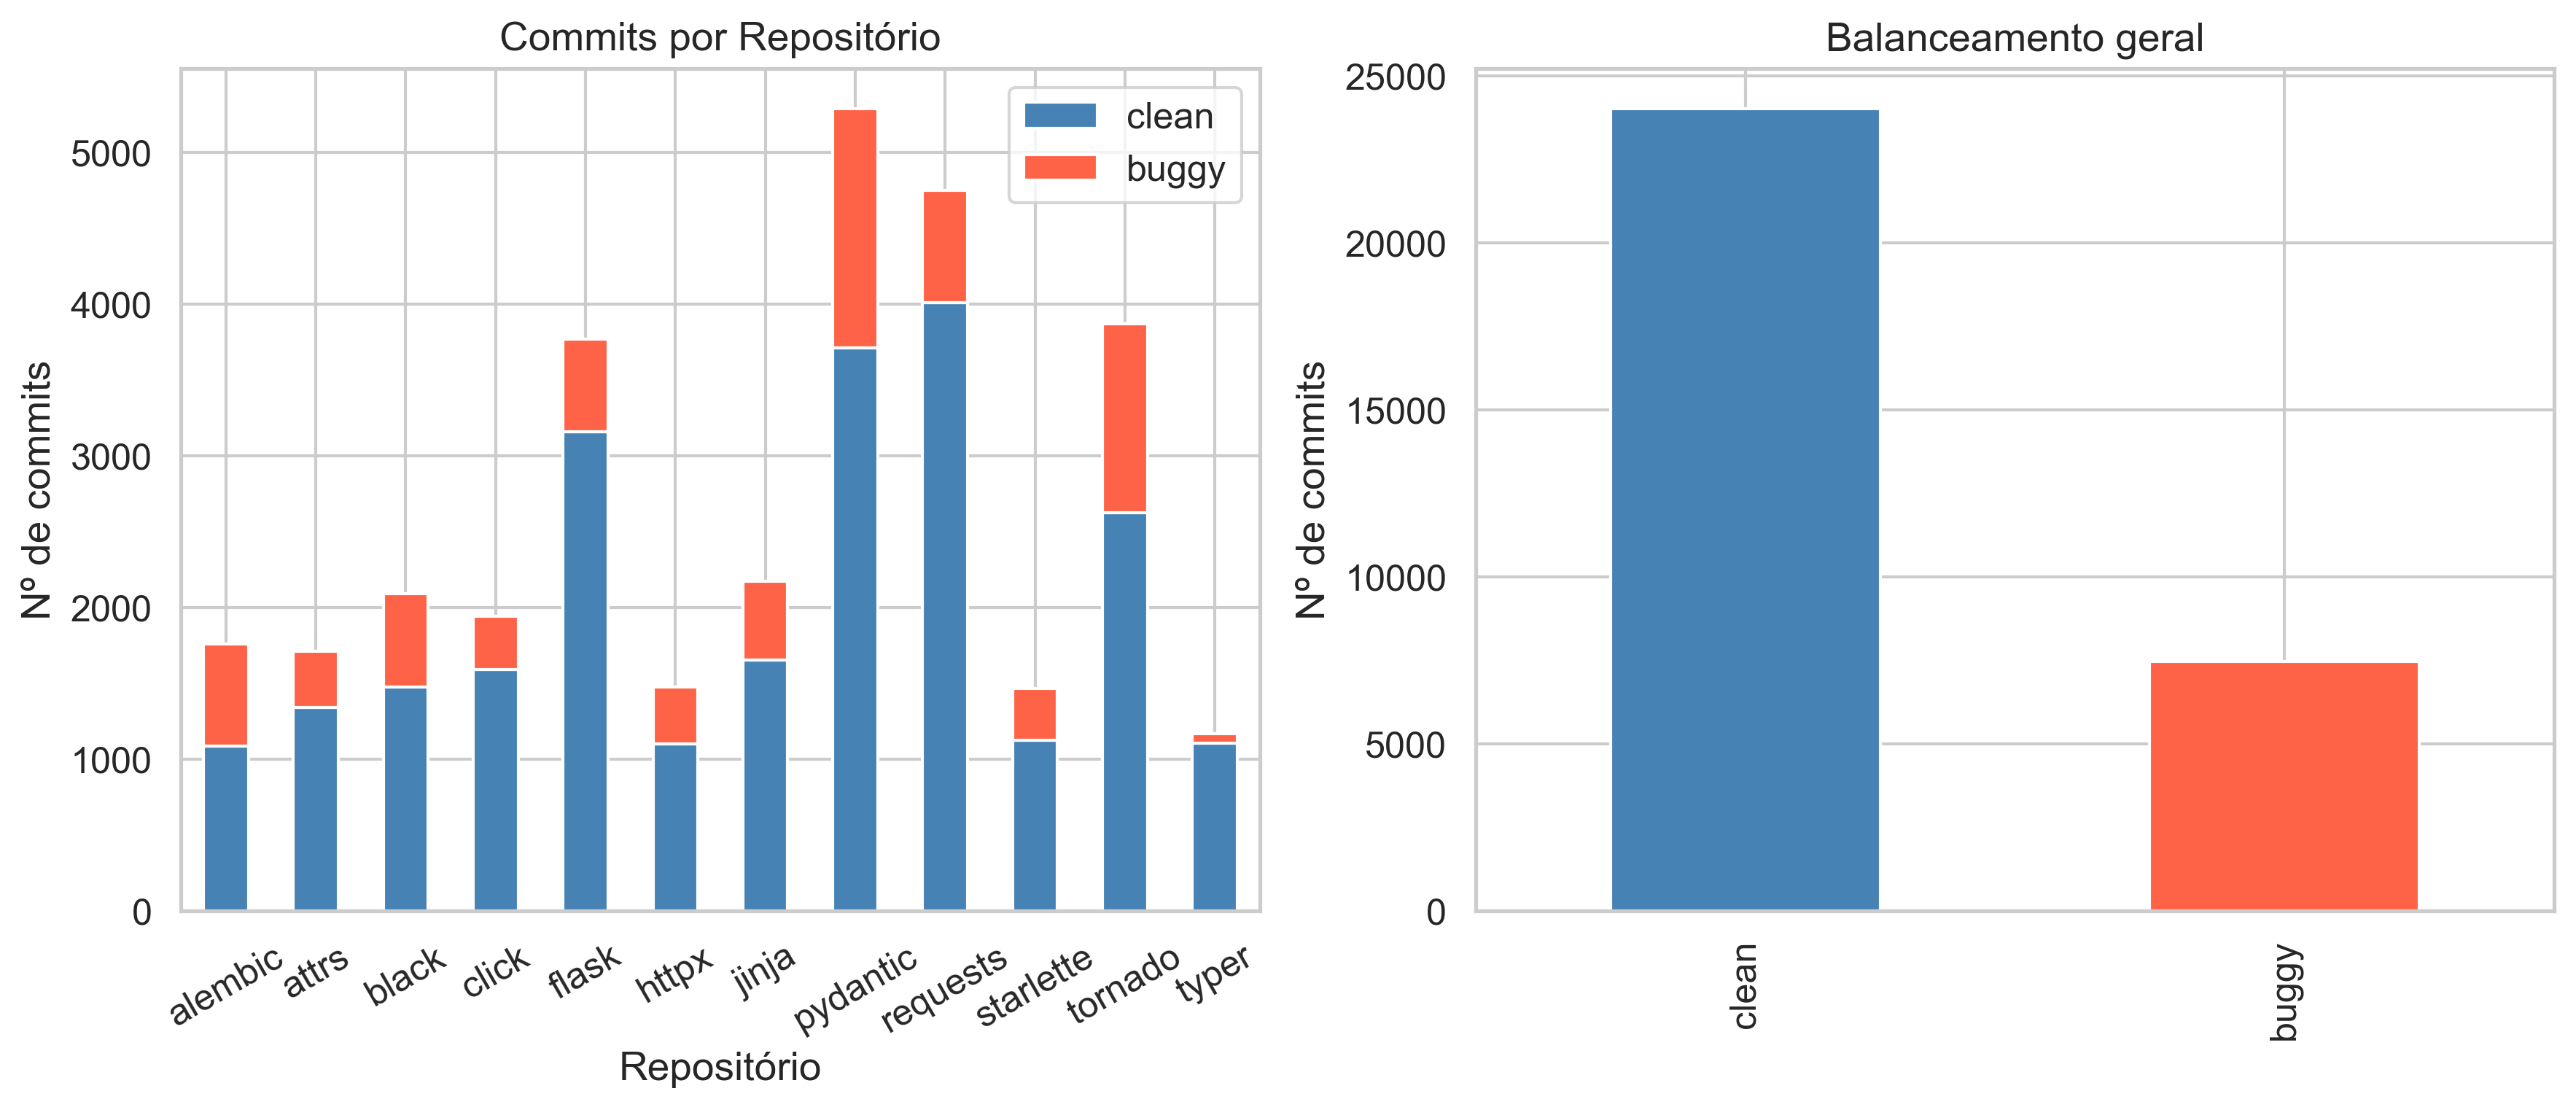
\includegraphics[width=\linewidth]{../output/figures/class_balance.png}
  \caption{Distribuição de commits buggy (vermelho) e limpos (azul) por repositório.}
  \label{fig:balance}
\end{figure}

As métricas apresentam distribuições fortemente assimétricas, conforme esperado para
métricas de código: LA tem média 51,5 e máximo 75.872; LT tem média 278 e máximo 18.968.
Após transformação $\log(x+1)$, as distribuições tornam-se mais adequadas para
os modelos lineares. A Figura~\ref{fig:dist} ilustra as distribuições das
principais features após transformação.

\begin{figure}[H]
  \centering
  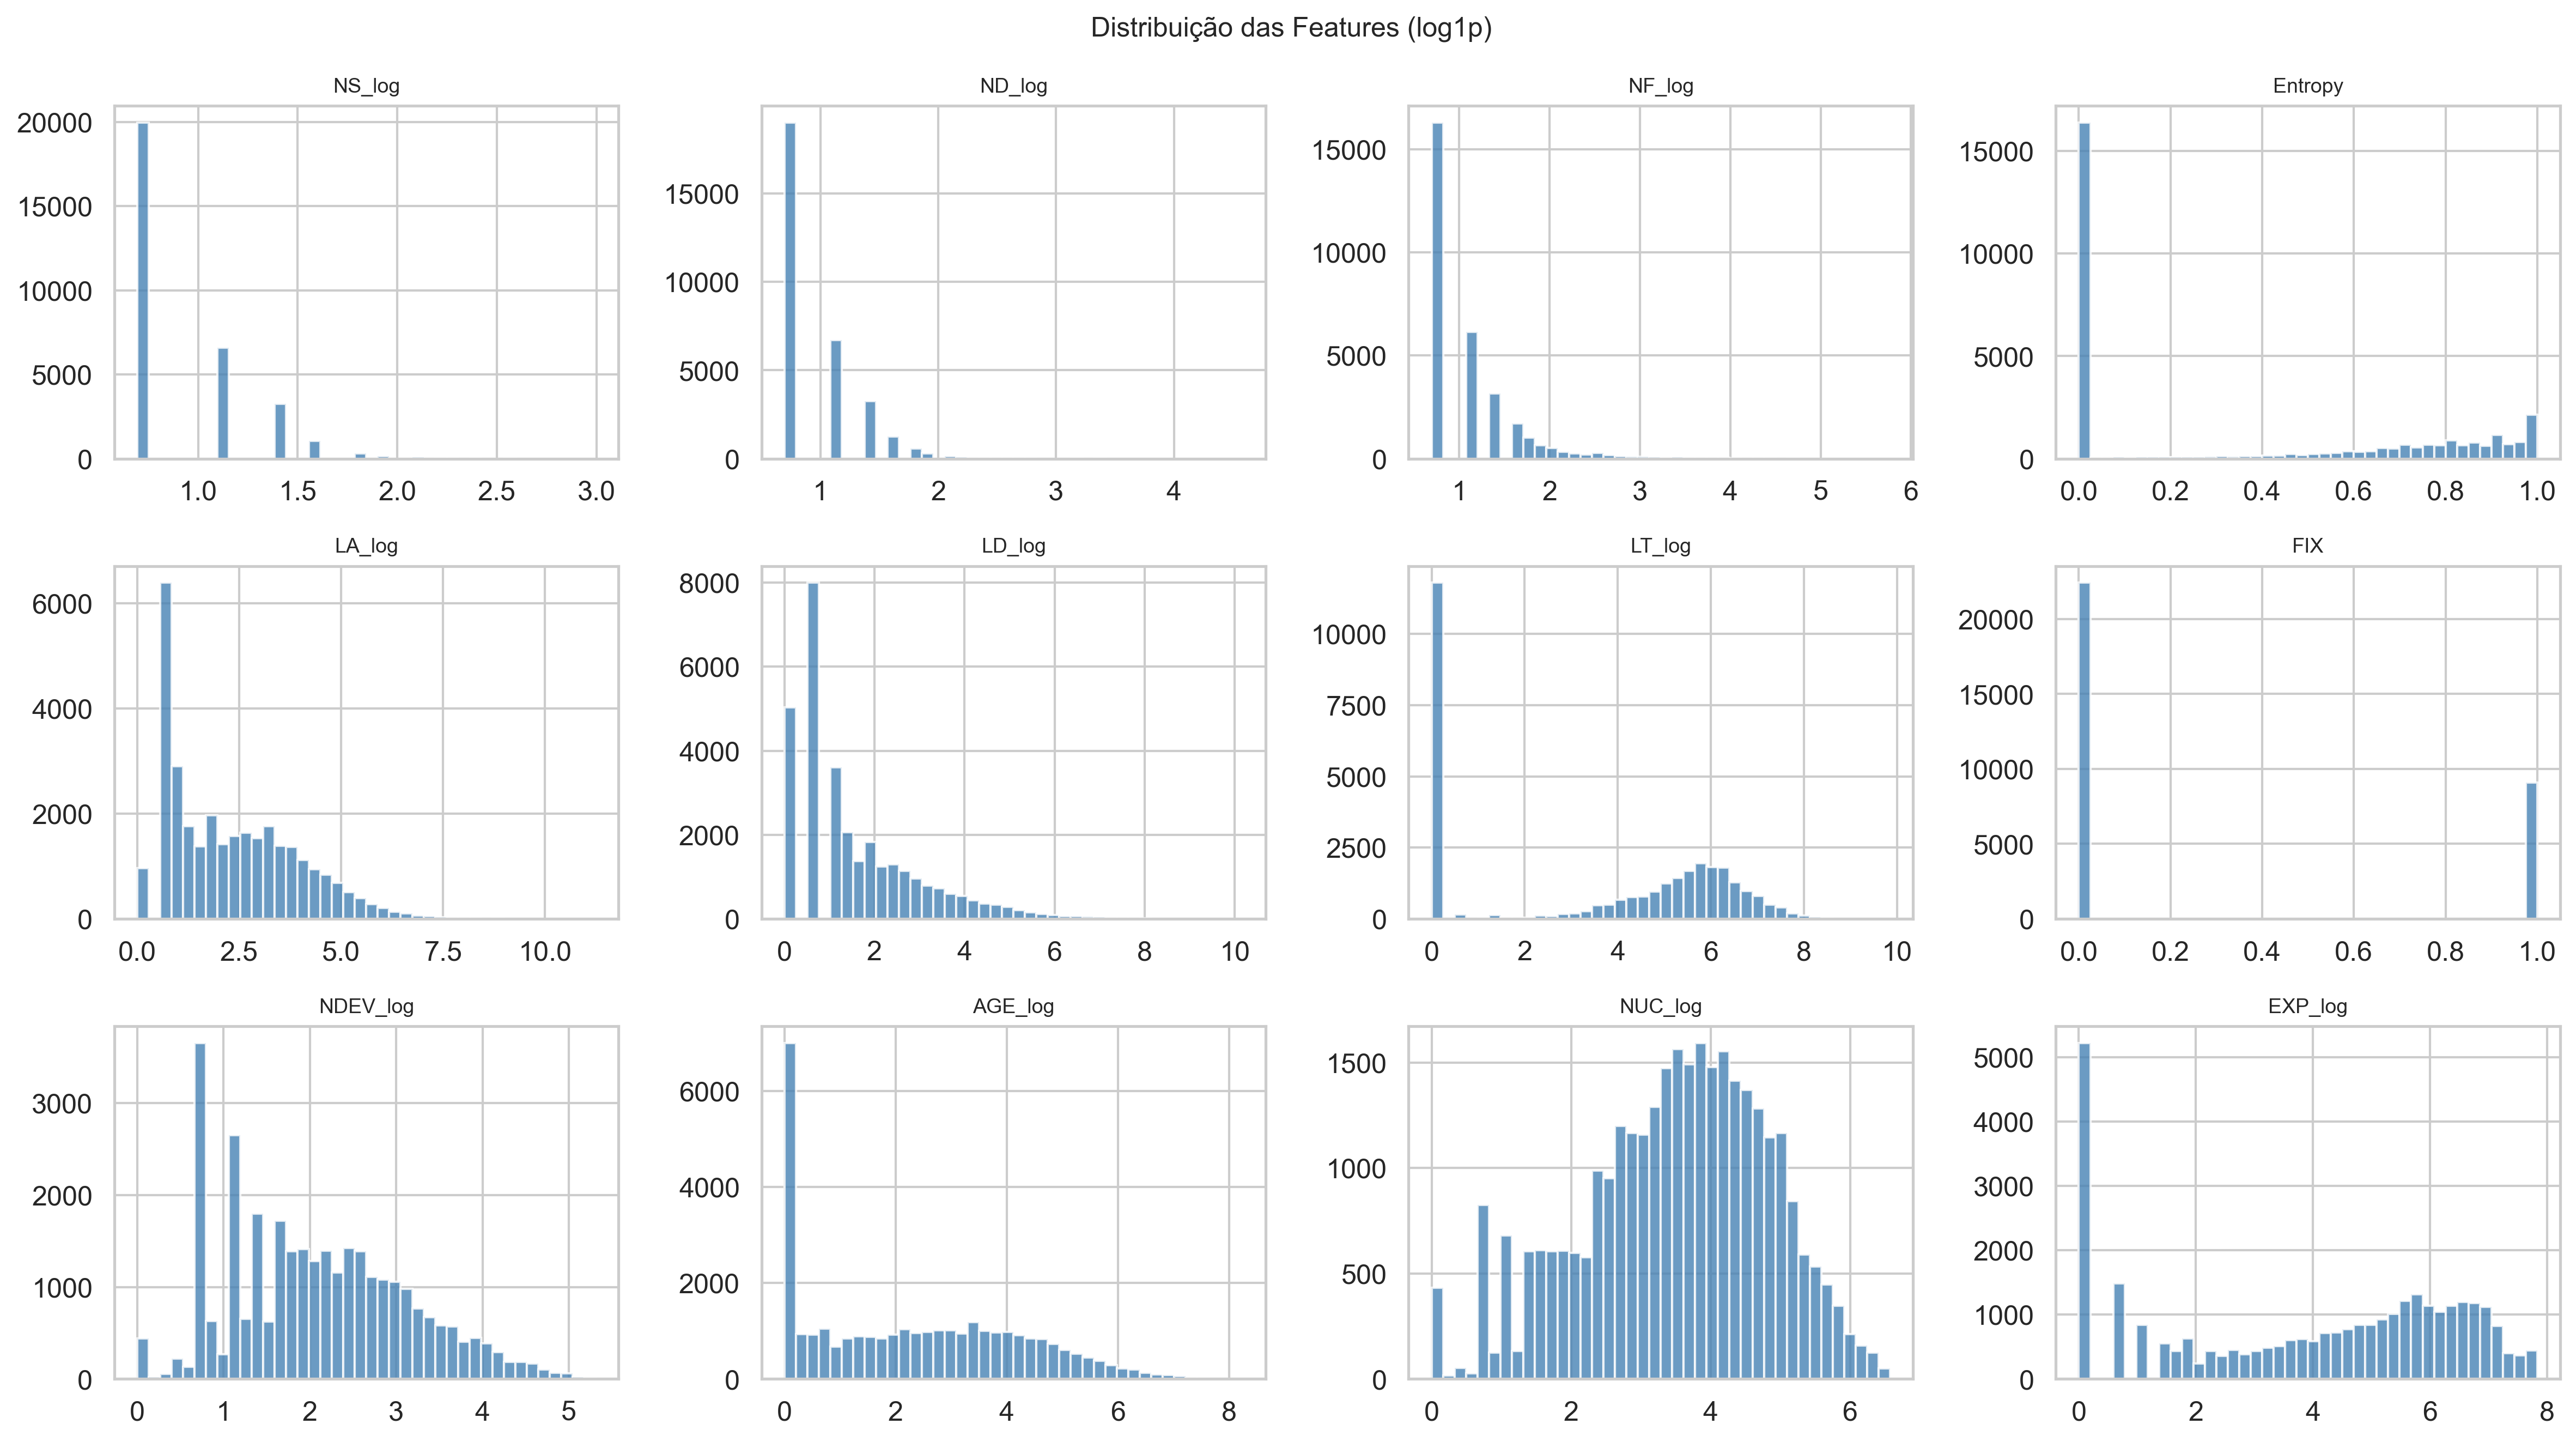
\includegraphics[width=\linewidth]{../output/figures/feature_distributions.png}
  \caption{Distribuição das 16 features após transformação $\log(x+1)$.}
  \label{fig:dist}
\end{figure}

\subsection{Correlação entre Features}

A Figura~\ref{fig:corr} apresenta o mapa de correlação de Spearman entre as features.
Observa-se alta correlação entre NF\_log e ND\_log ($\rho \approx 0{,}8$), indicando
que commits que tocam mais arquivos também tendem a modificar mais diretórios.
LA\_log e LD\_log são moderadamente correlacionados ($\rho \approx 0{,}5$), refletindo
que commits grandes tendem a adicionar e remover linhas simultaneamente.

\begin{figure}[H]
  \centering
  
\includegraphics[width=0.85\linewidth]{../output/figures/correlation_heatmap.png}
  \caption{Mapa de calor de correlação de Spearman entre features (log-transformadas).}
  \label{fig:corr}
\end{figure}

\subsection{Comparação de Modelos --- Split Temporal}

A Tabela~\ref{tab:temporal} apresenta os resultados no split temporal, que representa
o cenário real de uso do modelo. As curvas ROC e Precision-Recall são exibidas nas
Figuras~\ref{fig:roc} e~\ref{fig:pr}.

\begin{table}[H]
\centering
\caption{Resultados dos classificadores no split temporal (primário).}
\label{tab:temporal}
\begin{tabular}{lcccccc}
\toprule
\textbf{Modelo} & \textbf{Acc.} & \textbf{Prec.} & \textbf{Recall} & \textbf{F1} & \textbf{ROC-AUC} & \textbf{PR-AUC} \\
\midrule
Logistic Regression & 0,729 & 0,344 & \textbf{0,915} & 0,500 & \textbf{0,885} & \textbf{0,535} \\
Random Forest       & 0,778 & 0,385 & 0,833 & \textbf{0,526} & 0,881 & 0,512 \\
XGBoost             & 0,742 & 0,355 & 0,902 & 0,509 & 0,884 & 0,521 \\
LightGBM            & 0,751 & 0,361 & 0,884 & 0,513 & 0,880 & 0,517 \\
\bottomrule
\end{tabular}
\end{table}

\begin{figure}[H]
  \centering
  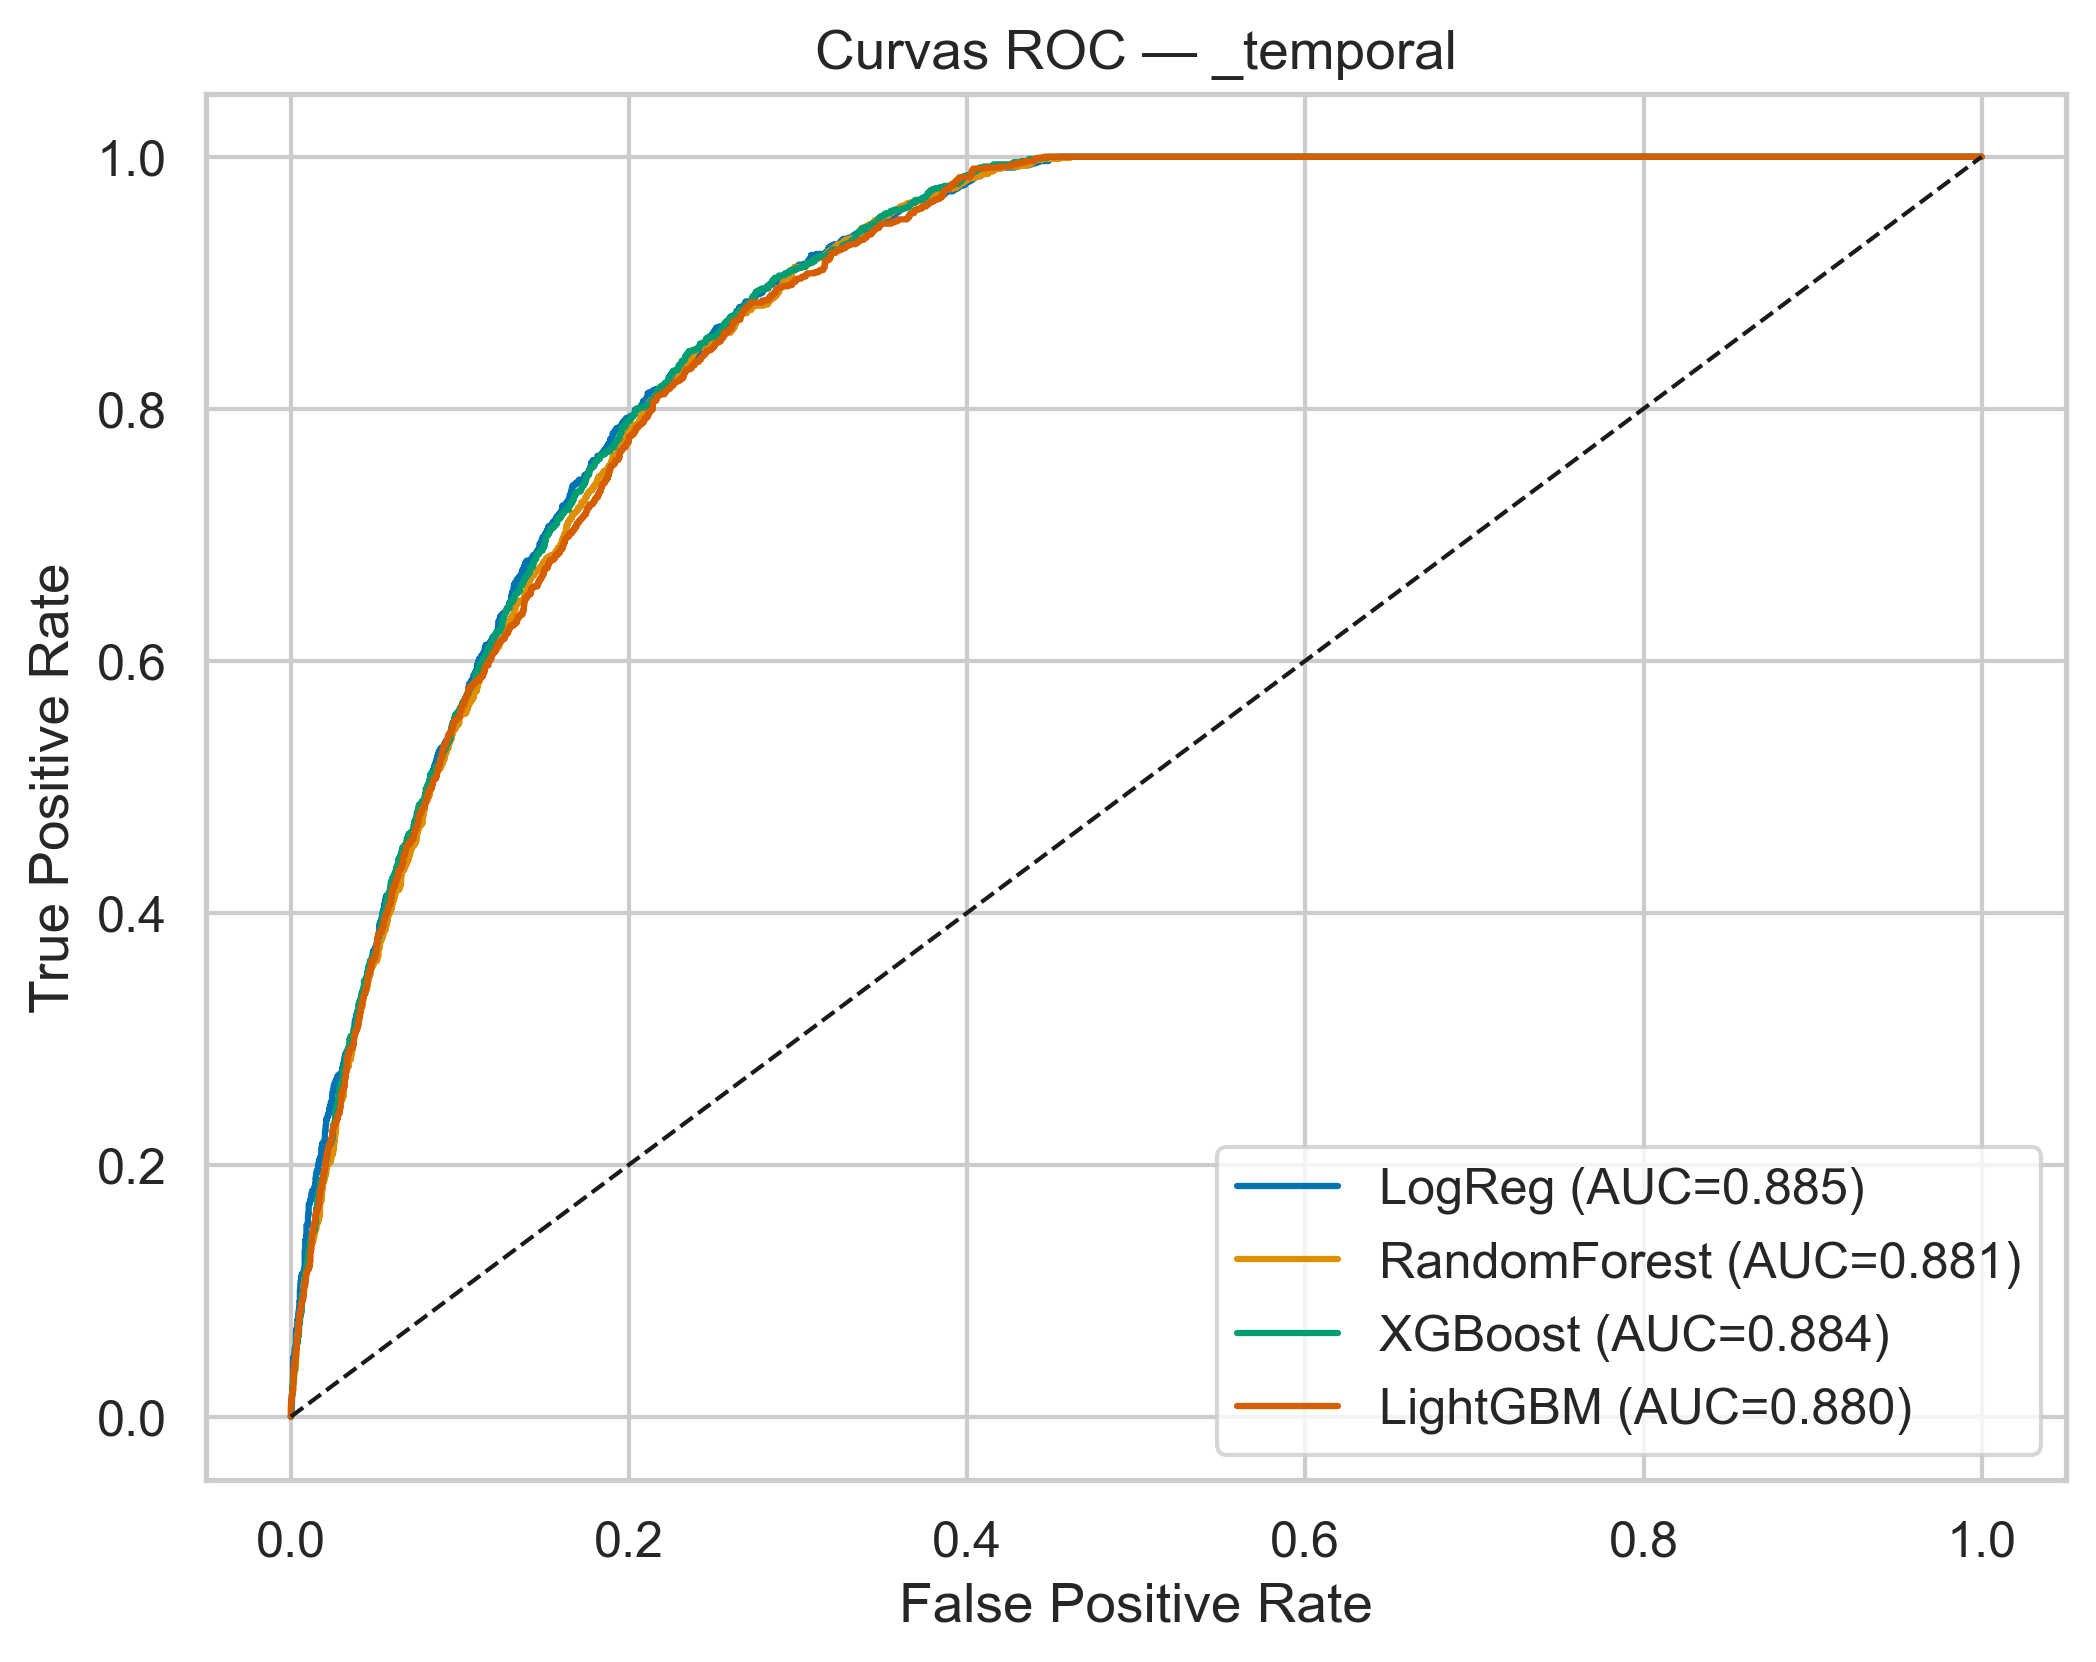
\includegraphics[width=0.85\linewidth]{../output/figures/roc_curves_temporal.png}
  \caption{Curvas ROC dos classificadores no split temporal.}
  \label{fig:roc}
\end{figure}

\begin{figure}[H]
  \centering
  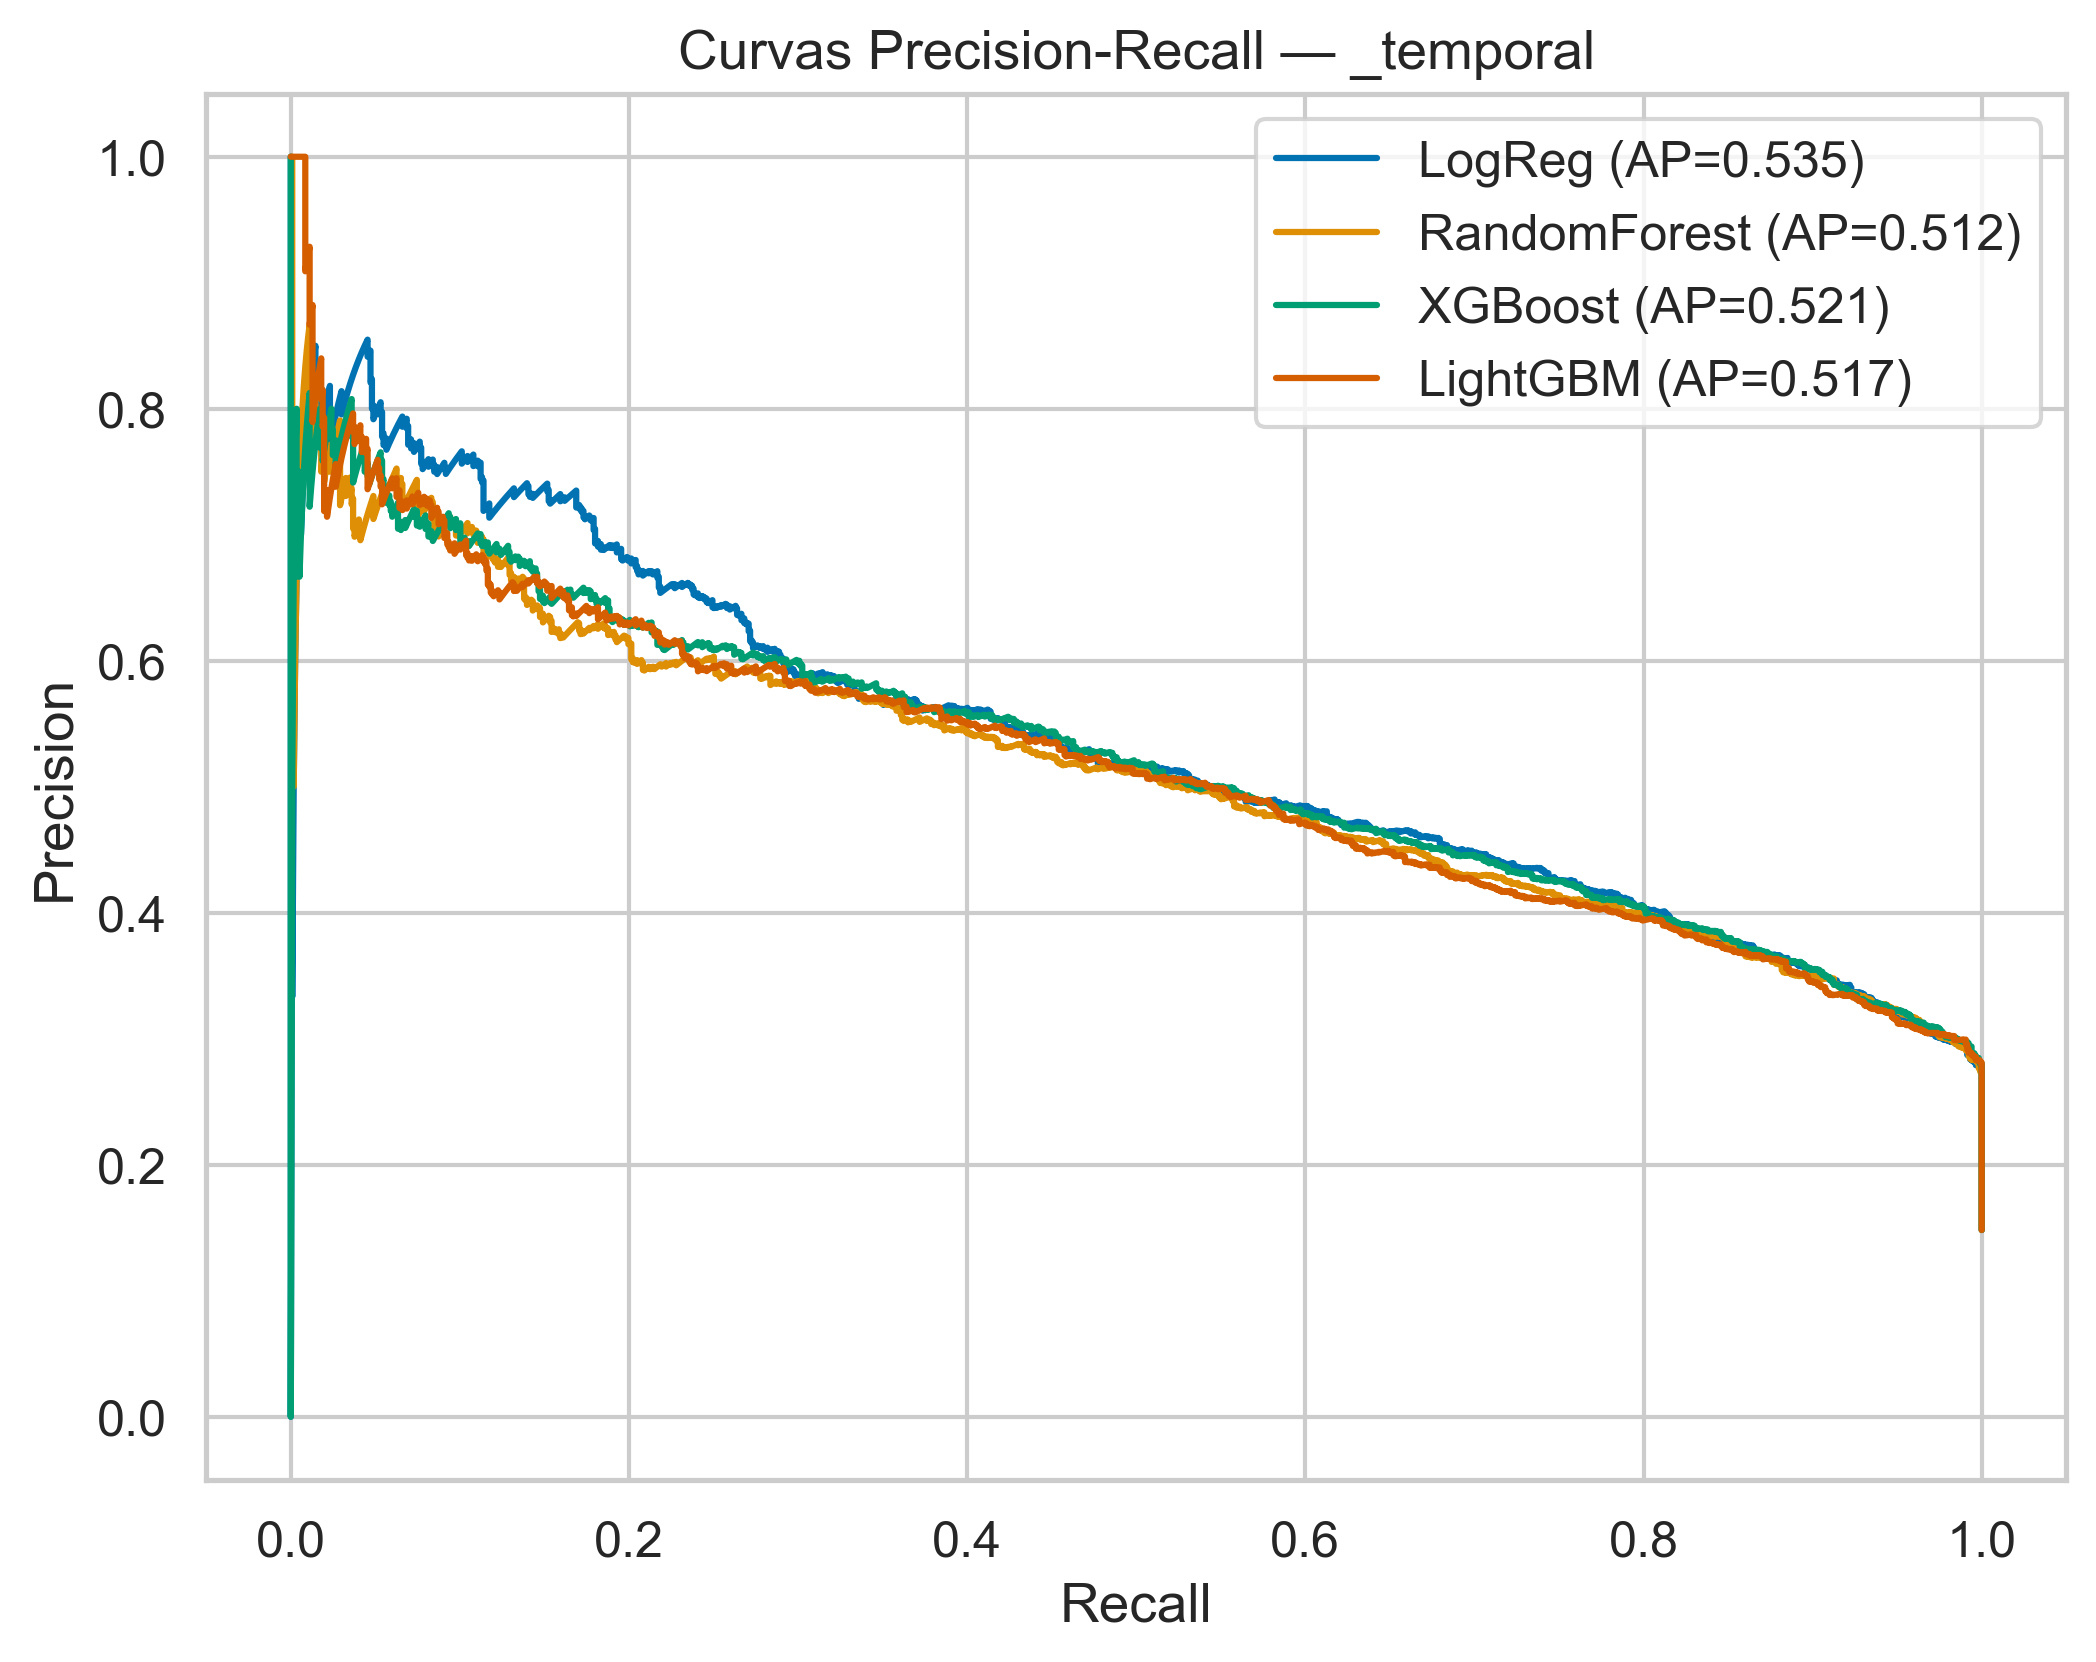
\includegraphics[width=0.85\linewidth]{../output/figures/pr_curves_temporal.png}
  \caption{Curvas Precision-Recall dos classificadores no split temporal.}
  \label{fig:pr}
\end{figure}

Todos os modelos atingem ROC-AUC próximo a 0,88, indicando boa capacidade de
ranqueamento dos commits por risco. O alto Recall da Regressão Logística (0,915)
é desejável em um sistema de alerta precoce, onde preferimos alertar sobre commits
limpos (falsos positivos) a deixar passar commits buggy (falsos negativos).
O Random Forest obteve o melhor F1 (0,526), oferecendo melhor equilíbrio entre
Precision e Recall.

\subsection{Importância de Features}

\begin{figure}[H]
  \centering
  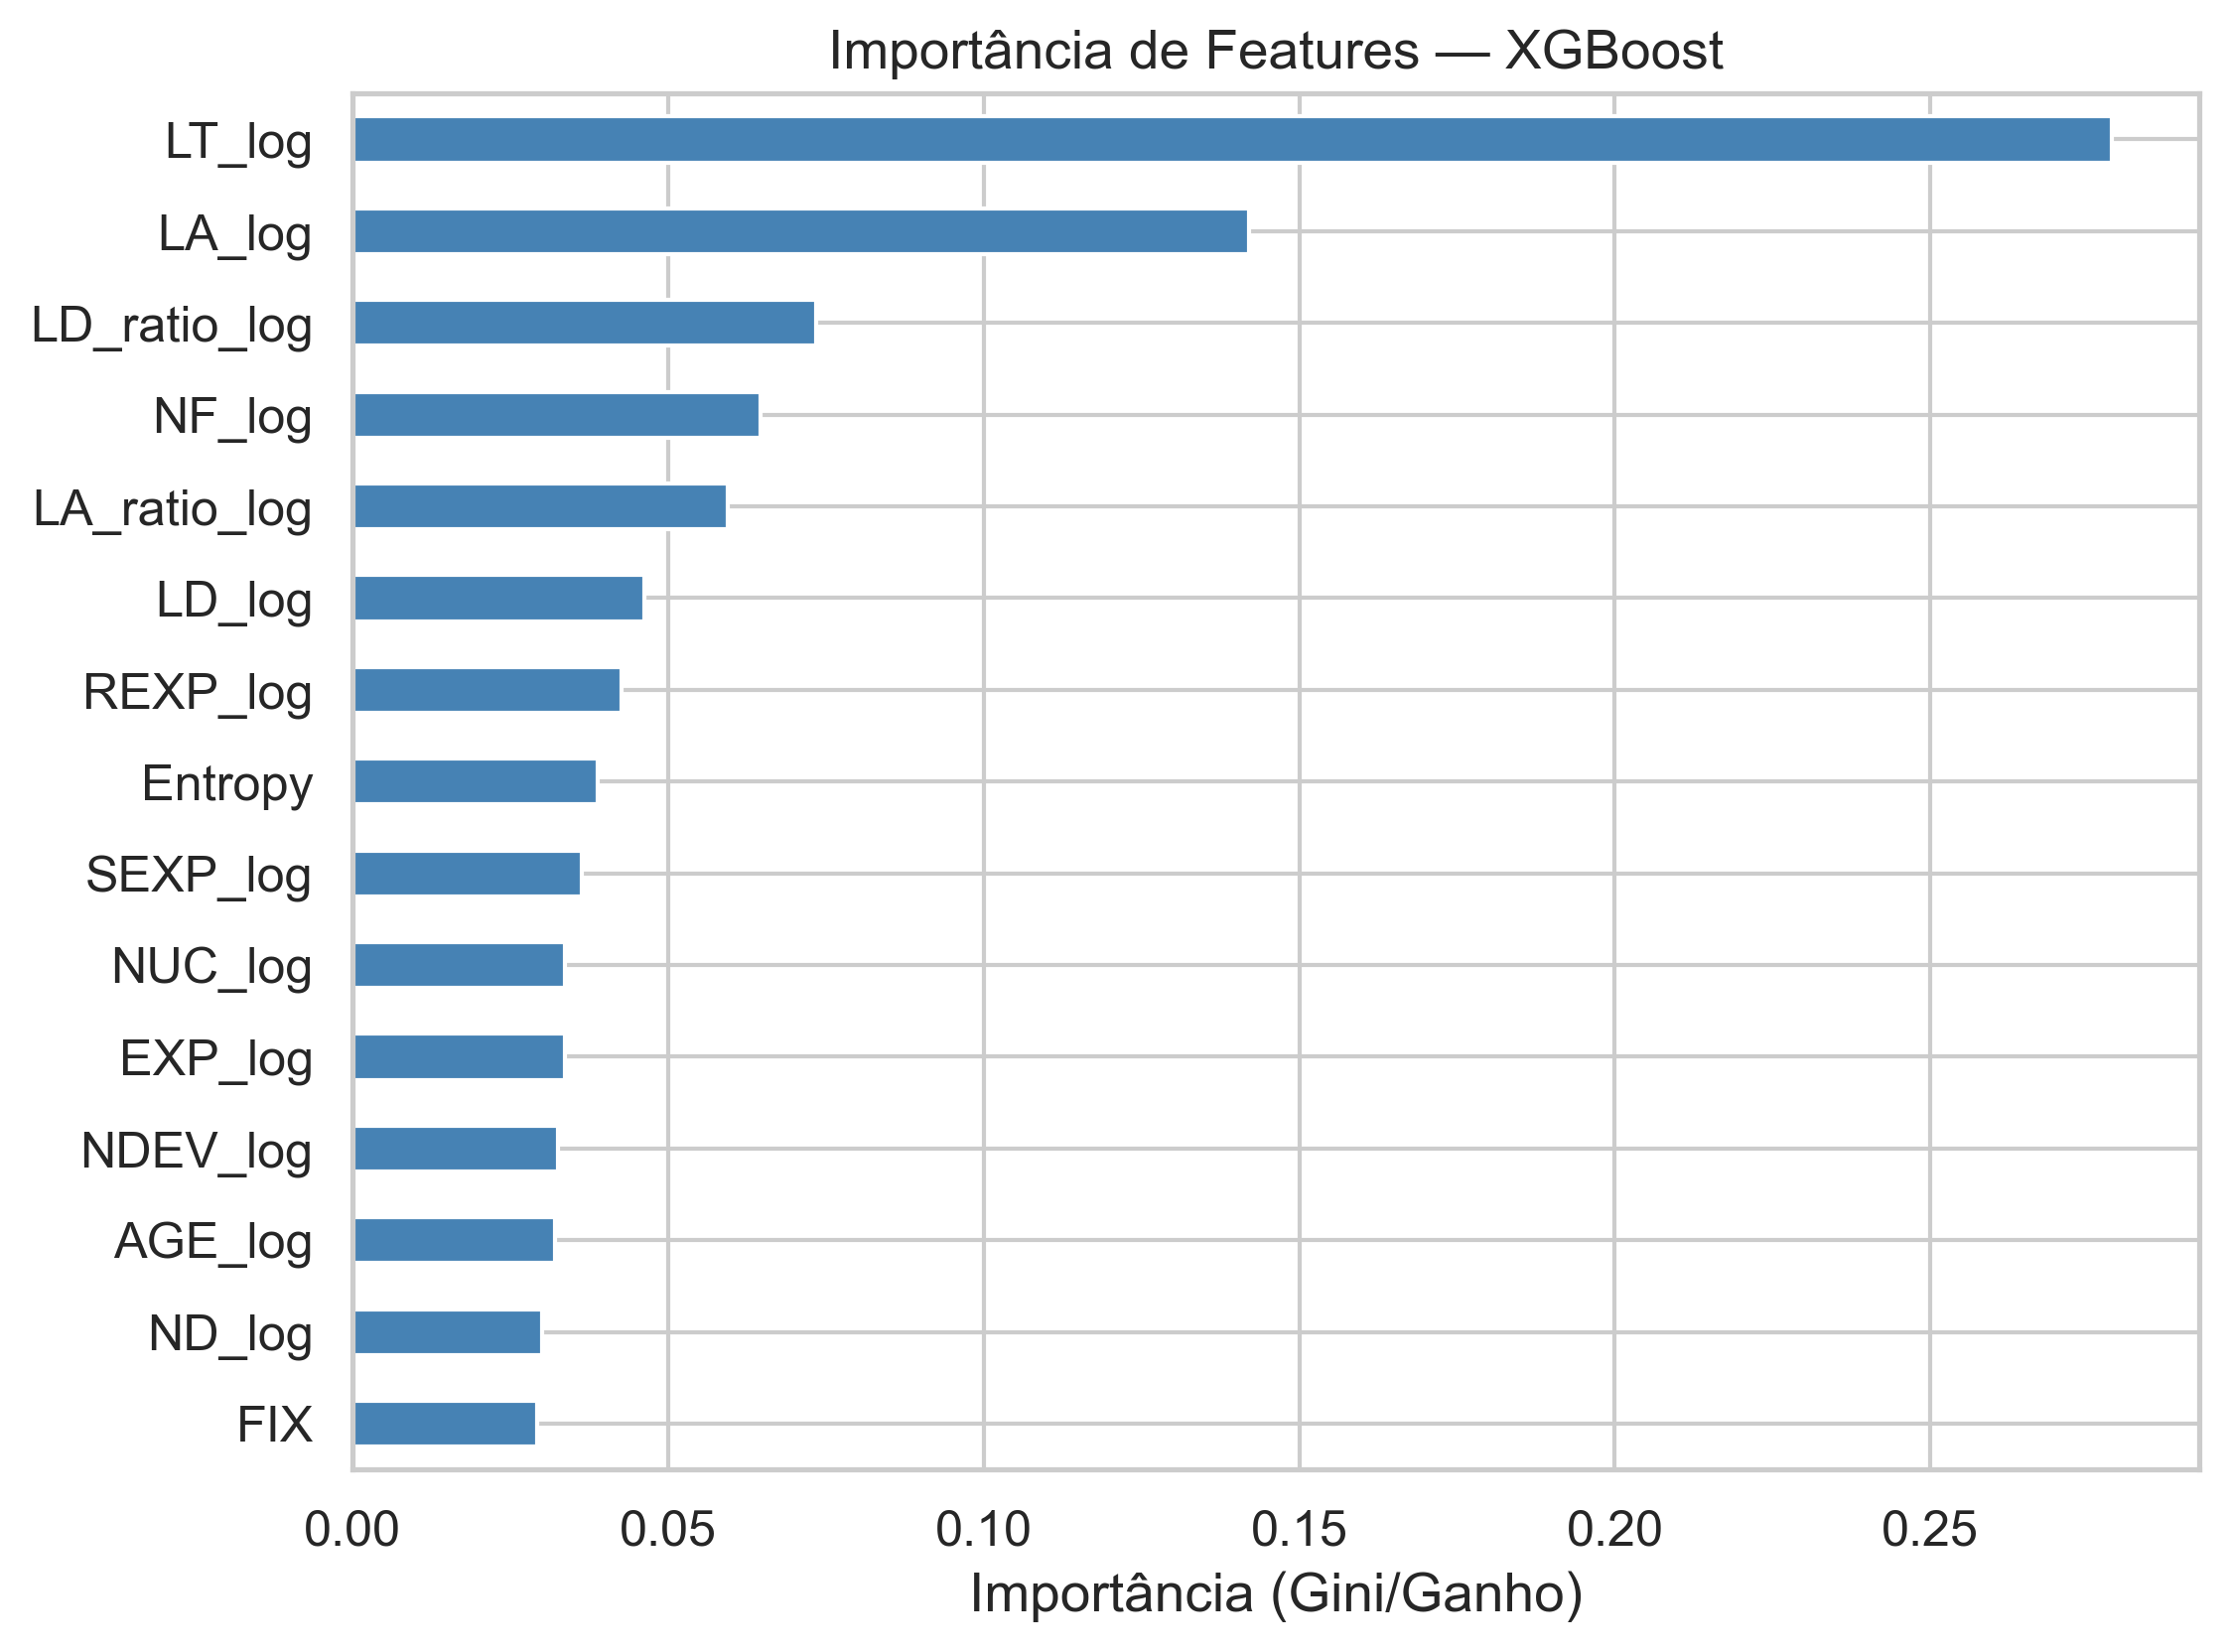
\includegraphics[width=0.85\linewidth]{../output/figures/feature_importance_xgboost.png}
  \caption{Importância de features no XGBoost (split temporal).}
  \label{fig:feat}
\end{figure}

A Figura~\ref{fig:feat} exibe a importância de features do XGBoost. A feature mais
relevante é \textbf{LT\_log} (tamanho do arquivo antes da mudança, 27,9\%),
seguida de \textbf{LA\_log} (linhas adicionadas, 14,2\%) e \textbf{LD\_ratio\_log}
(razão de linhas removidas, 7,3\%). Essa hierarquia é consistente com os achados de
Kamei~\textit{et al.}~\cite{kamei2013}, que também identificaram as dimensões de
tamanho e difusão como mais preditivas. Notavelmente, a feature FIX---derivada
diretamente do mecanismo de detecção de bugs---apresentou importância relativamente
baixa (2,9\%), o que mitiga a preocupação com vazamento de rótulo.

\subsection{Viés de Vazamento Temporal}

\begin{figure}[H]
  \centering
  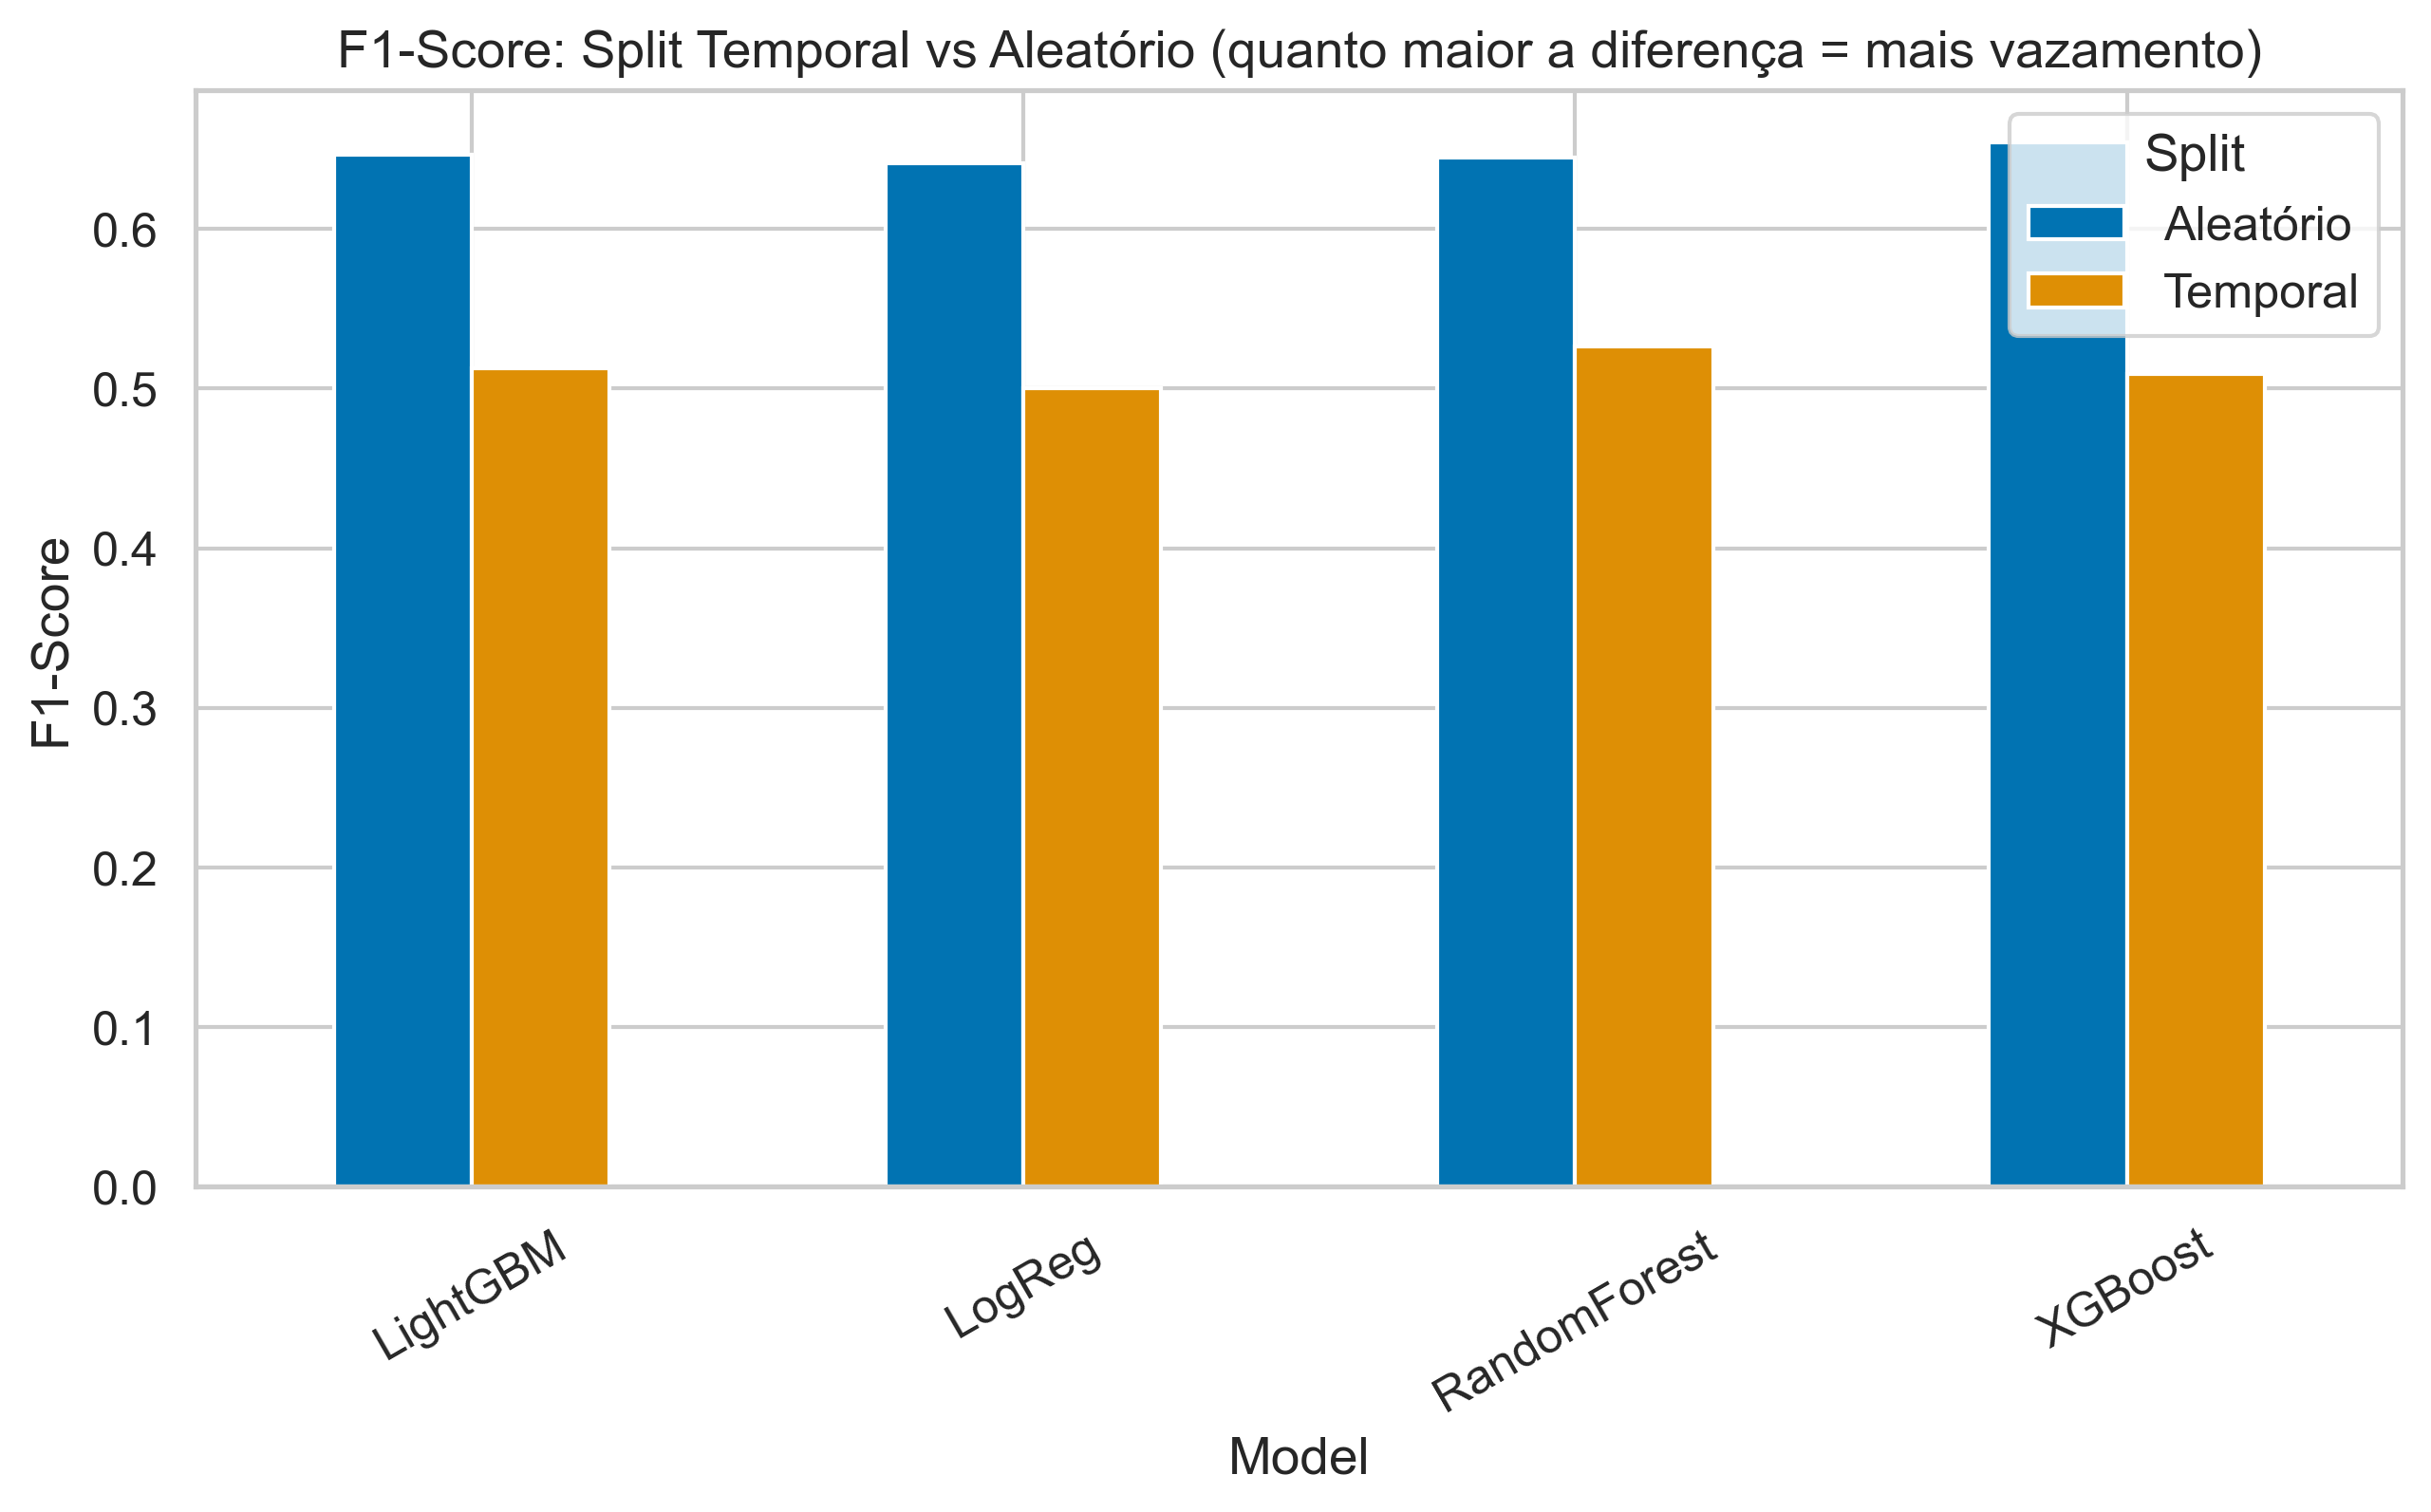
\includegraphics[width=0.85\linewidth]{../output/figures/time_vs_random_split.png}
  \caption{Comparação de F1-Score entre split temporal e aleatório. A diferença revela o viés de vazamento temporal.}
  \label{fig:leakage}
\end{figure}

A Figura~\ref{fig:leakage} e a Tabela~\ref{tab:random} ilustram o impacto do tipo de
divisão. No split aleatório, o XGBoost atinge F1 = 0,654 e PR-AUC = 0,709, valores
substancialmente superiores aos 0,509 e 0,521 obtidos no split temporal.
Esse aumento de $\approx$22\% no F1 representa uma superestimação sistemática do
desempenho real, causada pelo fato de que o modelo \textit{vê o futuro} ao ser
treinado com commits intercalados com o conjunto de teste.

\begin{table}[H]
\centering
\caption{Resultados no split aleatório (comparação).}
\label{tab:random}
\begin{tabular}{lcccccc}
\toprule
\textbf{Modelo} & \textbf{Acc.} & \textbf{Prec.} & \textbf{Recall} & \textbf{F1} & \textbf{ROC-AUC} & \textbf{PR-AUC} \\
\midrule
Logistic Regression & 0,772 & 0,511 & 0,858 & 0,641 & 0,883 & 0,671 \\
Random Forest       & 0,811 & 0,583 & 0,720 & 0,645 & 0,890 & 0,703 \\
XGBoost             & 0,797 & 0,550 & 0,808 & \textbf{0,654} & \textbf{0,890} & \textbf{0,709} \\
LightGBM            & 0,791 & 0,540 & 0,805 & 0,647 & 0,890 & 0,709 \\
\bottomrule
\end{tabular}
\end{table}

Destaca-se que o ROC-AUC permanece quase inalterado entre os dois splits
($\approx$0,88 em ambos), sugerindo que a capacidade de ranqueamento do modelo
é genuína. A queda no F1, porém, revela que a distribuição temporal diferente entre
treino (26,7\% buggy) e teste (14,8\% buggy) prejudica a calibração do limiar de decisão.

\subsection{Regressão de Churn}

Como tarefa complementar, treinamos modelos de regressão para prever o churn
$\log(LA+LD+1)$. O Random Forest obteve RMSE = 0,026 e MAE = 0,004, desempenho
muito superior ao Ridge (RMSE = 0,289, MAE = 0,168), confirmando que a relação
entre as features de histórico/experiência e o volume de mudanças é altamente
não-linear.

\subsection{Ameaças à Validade}

\textbf{Validade interna:} o SZZ-lite pode gerar falsos positivos ao associar
refatorações e ajustes cosméticos como \textit{bug-inducing}. A feature FIX é
derivada do mesmo mecanismo de detecção, representando potencial vazamento de
rótulo; sua baixa importância (2,9\%) mitiga esse risco.
\textbf{Validade externa:} limitamo-nos a 12 projetos Python de código aberto de
médio porte. Os resultados podem não se generalizar para projetos em outras linguagens,
de grande escala ou de desenvolvimento corporativo fechado.
\textbf{Maturação:} commits recentes podem ser erroneamente classificados como limpos
por ainda não terem sido associados a correções; mitigamos com a janela de 180 dias,
embora commits entre 30 e 180 dias possam ainda estar sujeitos a esse viés~\cite{dacosta2017}.

% ─────────────────────────────────────────────────────────────────────────────
\section{Conclusão}
\label{sec:conclusao}

Neste trabalho apresentamos uma abordagem completa e reproduzível de Just-In-Time
defect prediction para 12 repositórios Python reais. Mineramos 31.492 commits com
PyDriller, extraímos as 14 métricas Kamei e rotulamos os commits bug-inducing via
SZZ-lite, obtendo um dataset público com 23,8\% de exemplos positivos.

Comparamos quatro classificadores com otimização de hiperparâmetros. No cenário
temporal, que reflete o uso real do modelo, o Random Forest obteve o melhor
F1-Score (0,526) e a Regressão Logística o melhor ROC-AUC (0,885).
A análise comparativa entre splits revelou um viés de vazamento temporal de
$\approx$22\% no F1 quando a ordenação cronológica é ignorada---um achado relevante
para a comunidade de MSR, que frequentemente avalia modelos com divisão aleatória.
A feature LT (tamanho do arquivo antes da mudança) foi a mais preditiva,
seguida de LA (linhas adicionadas), em linha com a literatura.

Como trabalho futuro, planejamos expandir para mais repositórios e linguagens,
incorporar métricas de revisão de código (comentários e rejeições de pull requests),
avaliar abordagens de aprendizado profundo e aplicar o RA-SZZ~\cite{dacosta2017}
para rotulagem mais precisa.

% ─────────────────────────────────────────────────────────────────────────────
\bibliographystyle{sbc}
\bibliography{referencias}

\end{document}
